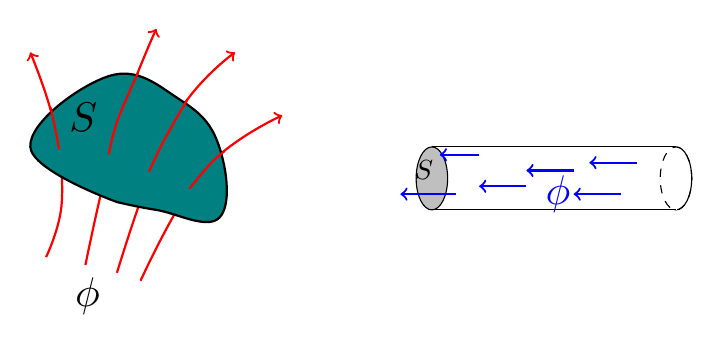
\begin{tikzpicture}

\draw [->, thick, red] plot[smooth, tension=.7] coordinates {(-2.6,-0.4) (-2.4,0.3) (-2.5,1.3) (-2.8,2.2)};
\draw [->, thick, red] plot[smooth, tension=.7] coordinates {(-2.1,-0.5) (-1.7,1.2) (-1.2,2.5)};
\draw [->, thick, red] plot[smooth, tension=.7] coordinates {(-1.7,-0.6) (-1,1.3) (-0.2,2.2)};
\draw [->, thick, red] plot[smooth, tension=.7] coordinates {(-1.4,-0.7) (-0.6,0.7) (0.4,1.4)};
\draw [fill=teal, thick] plot[smooth, tension=.7] coordinates {(-1.7,0.3) (-1.2,0.2) (-0.4,0.1) (-0.4,1) (-0.9,1.6) (-1.8,1.9) (-2.8,1) (-1.7,0.3)};

\draw  [red, thick]plot[smooth, tension=.7] coordinates {(-2.4,0.6)};
\draw  [red, thick]plot[smooth, tension=.7] coordinates {(-2.4338,0.9679) (-2.4722,1.173) (-2.5413,1.5002)};
\draw  [red, thick]plot[smooth, tension=.7] coordinates {(-1.8056,0.9038) (-1.6902,1.3397) (-1.4332,1.9387)};
\draw  [red, thick]plot[smooth, tension=.7] coordinates {(-1.2927,0.6859) (-1.0876,1.1089) (-0.8086,1.5955)};
\draw  [red, thick]plot[smooth, tension=.7] coordinates {(-0.7799,0.4679) (-0.5107,0.7884) (-0.3303,0.9488)};
\node at (-2.0748,-0.8911) [scale=1.5] {$\phi$};
\node at (-2.1261,1.3765) [scale=1.5]{$S$};

\draw  (5.4,0.6) ellipse (0.2 and 0.4);
\draw [fill,white] (2.3,1) rectangle (5.4,0.2);
\draw  [fill=lightgray](2.3,0.6) ellipse (0.2 and 0.4);
\draw (2.3,1) -- (5.4,1);
\draw (2.3,0.2) -- (5.4,0.2);
\draw  [dashed](5.4,0.6) ellipse (0.2 and 0.4);
\draw [blue, ->, thick](4.9,0.8) -- (4.3,0.8);
\draw [blue, ->, thick](4.7,0.4) -- (4.1,0.4);
\draw [blue, ->, thick](4.1,0.7) -- (3.5,0.7);
\draw [blue, ->, thick](3.5,0.5) -- (2.9,0.5);
\draw [blue, ->, thick](2.9,0.9) -- (2.4,0.9);
\draw [blue, ->, thick](2.6,0.4) -- (1.9,0.4);
\node [blue, scale=1.5] at (3.9,0.4) {$\phi$};
\node at (2.2,0.7) {$S$};
\end{tikzpicture}